\section{Introduction}




=======
The recent commercial availablity of relatively cheap mobile robots such as
Baxter and the UBR 1 has created a very real possiblity for widespread
application of robotics to mobile manipulation tasks.  There are huge economic
gains to be had from the deployment of robotics in a variety of settings that
range from homes to factories.  However, getting robots to execute complex,
goal-directed tasks in such unstructured settings remains a major challenge.

In particular, deformable object manipulation presents an interesting challenge.
These problems are characterized by state and action spaces that are high-dimensional 
and continuous and direct solutions require reasoning about dynamics of complex object 
through contact.
Determing a correct underlying representation of these objects is itself a difficult problem,
and current approaches require complicated task specific implementations.

Learning from demonstrations provides a way to sidestep these issues: rather
than starting from scratch in each scenario, we generalize from an expert
demonstration.  If this generalization can be done robustly, adapting an example
trajectory to a new scene gives an easy way for laypeople to provide custom
solutions a wide variety of tasks well beyond the state-of-the-art.

A recent approach makes use of \emph{trajectory transfer} through the use of
non-rigid registration to solve this problem.  Trajectory transfer fits a
function $f:\mathbb{R}^3 \rightarrow \mathbb{R}^3$ that warps a demonstration
scene to a novel setting.  The demonstrated trajectory is warped with this
function and the result is executed in the current scene.  This has been shown
to be effective for many complex task, including knot-tying and suturing
\cite{Schulmanetal_ISRR2013, Schulmanetal_IROS2013}.

Of course, a single demonstration cannot be expected to cover all possible scenarios.
The natural solution to this is to use a library of demonstrations.
In addition to increasing the number of states we can adapt to, trajectory libraries
enable execution of complex tasks beyond mere cloning of demonstrations by sequencing 
several trajectory generalizations.

However, realizing these benefits requires a robust technique to select a good trajectory to
transfer.
This is not an easy task.
Certain trajectories will generalize better than others, and particular sequences of 
demonstrations may perform tasks more efficiently than others.
Furthermore, the existence of poor or brittle demonstrations can very negatively 
effect performance.
Na\"{\i}ve approaches that simply use the goodness of the warping fit discard much of this information and often fail to accomplish tasks that would be possible with a different sequence of trajectories.

\begin{figure}[t]
  \centering
    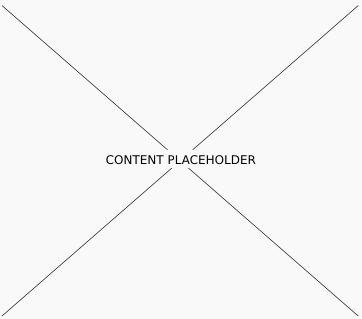
\includegraphics[width=0.9\linewidth]{figures/placeholder.png}
  \caption{Cute picture of robot tying knot}
  \label{fig:frontfig}
\end{figure}

In this paper, we present a solution to the demonstration selection problem that
can account for the variability in robustness of demonstrations and the
sequential nature of our tasks.  Given a set of demonstrations and a method for
applying them to similar situations, we construct a discrete action abstract
Markov decision process (MDP).  Each action in this MDP is associated with a
demonstration, and our transition function is defined as applying trajectory
transfer to generalize that demonstration.

This construction allows us to learn a Q function from example sequences of 
state and demonstration pairs.
Our Q-function learning is done through a novel Learning from Demonstrations
technique that accounts for both the optimality of the expert trajecotries and the
sequenatial nature of the task.
We call this approach Max-Margin Q Learning, {\sc mmql}.

Our approach relies only on features which are completely task 
agnostic and can be applied to any problem where trajectory transfer applies. 
We investigate the utility of this approach in a challenging knot-tieing scenario 
and show that the greedy application of our learned policy strongly outperforms the 
\citet{Schulmanetal_ISRR2013}'s nearest-neighbor method on a challenging distribution of 
problems. 
We leverage the fact that we learn a Q function representation of our policy (as 
opposed to a direct mapping from features to actions) to use a beam search to get 
near perfect performance in this task.
Finally, we present a method for bootstrapping, though a process we call leave-one-out labeling, that enables us to apply {\sc mmql} with no additional human supervision beyond the initial demonstrations.

The rest of this paper is organized as follows: first, we review related work in
the field and discuss what differentiates our method. Next, we provide relevant
technical background for our method. We then provide a formal formulation of the
trajectory selection problem as a max-margin Q-learning problem, as well as a
discussion of the various features and policies that can be used with this
framework. We present experimental results in a knot-tying setting and provide
results that show that our learned policy can successfully tie a knot
significantly more often than the na\"{\i}ve nearest-neighbor approach. Finally,
we conclude with a summary of our work and a discussion of future work.
